\documentclass{classrep}
\usepackage[utf8]{inputenc}
\usepackage{color}
\usepackage{enumitem}
\usepackage{graphicx}
\usepackage{amsmath}
\usepackage{float}


\studycycle{Informatyka, studia dzienne, I st.}
\coursesemester{VI}

\coursename{Sztuczna Inteligencja i Systemy Ekspertowe}
\courseyear{2019/2020}

\courseteacher{dr inż. Krzysztof Lichy}
\coursegroup{wt., 12:15}

\author{
\studentinfo{Mateusz Walczak}{216911} \and
\studentinfo{Konrad Kajszczak}{216790}
}

\title{Zadanie 2: Sieć neuronowa służąca do korygowania pomiaru systemu lokalizacji}

\begin{document}
\maketitle

\section*{Wprowadzenie}
Celem zadania było zaprojektowanie i zaimplementowanie sieci neuronowej, która pozwoli na korygowanie błędów uzyskanych z systemu pomiarowego. Projektując sieć neuronową należało odpowiednio dobrać \cite{zadanie}:

\begin{itemize}[label=$\bullet$\scshape\bfseries]
\item liczbę warstw,
\item liczebność neuronów w poszczególnych warstwach,
\item funkcje aktywacji,
\item liczbę próbek z poprzednich chwil czasowych.
\end{itemize}

\section{Opis architektury sieci neuronowej}

W tym rozdziale rozpoczniemy od opisu działania naszego programu oraz drogi jaką przebyliśmy, aby znaleźć taką sieć neuronową, która pozwoli na skuteczne korygowanie błędów uzyskanych z systemu pomiarowego. Nastepnie skoncetrujemy się na opisie architektury tej sieci neuronowej, która okazała się najskutecznniejsza. 

\subsection{Historia wyboru odpowiedniej architektury sieci neuronowej}

Nasz program został napisany w języku $Java$, bez wykorzystania wysokopoziomowych bibliotek do tworzenia sieci neuronowych.
Program został napisany w taki sposób, aby w zależności od ustawień, tworzyć, inicjować a następnie przeprowadzać proces nauki dla sieci neuronowych o różnych liczbach nauronów w poszczególnych warstwach a także różnych liczbach próbek z poprzednich chwil czasowych.\newline 

Po wielu nieudanych próbach poprawy błędów uzyskanych z systemu pomiarowego, z wykorzystaniem sieci 2-warstwowych ($n$ neuronów w 1 warstwie i 2 neurony w warstwie wyjściowej), zdecydowano się na implementcję 3-warstowej sieci nueronowej.\newline

Nasza aplikacja buduje 3-warstową sieć neuronową na podstawie trzech parametrów, które na potrzeby tego sprawozdania będziemy nazywać $n_1$, $n_2$ oraz $p$. Kolejno, stanowią one:

\begin{itemize}[label=$\bullet$\scshape\bfseries]
\item $n_1$ - liczba neuronów w pierwszej warstwie sieci,
\item $n_2$ - liczba neuronów w drugiej warstwie sieci,
\item $p$ - liczbę próbek z poprzednich chwil czasowych wykorzystywanych przez sieć neuronową.
\end{itemize}

W tym miejscu warto wspomnieć o tym, że trzecia warstwa za każdym razem składała się z 2 neuronów, ponieważ nasza sieć musi mieć 2 wyjścia, aby spełniała warunki zadania (powinna zwracać współrzędną x-ową i y-ową dla danej próbki pomiarowej).\newline

Warstwa trzecia (wyjściowa) posiadała identycznościową funkcję aktywacji. Warstwy pierwsza i druga zaś funkcję hiperboliczną (tangens hiperboliczny), określoną wzorem:

\begin{equation}
\operatorname{tgh} x = \frac{\sinh x}{\cosh x} = \frac{e^x - e^{-x}}{e^x + e^{-x}}.
\end{equation}\newline

Wszystkie wagi, dla każdego z neuronów we wszystkich 3 warstwach, inicjalizowano wartością losową, należącą do przedziału $\langle-1; 1\rangle$.\newline

Program uruchamiano dla różnych kombinacji parametrów $n_1$, $n_2$ oraz $p$. W każdej z kombinacji powtarzano eksperymenty kilkukrotnie, w poszukiwaniu najbardziej optymalnego rozwiązania. Wartości osiągane przez poszczególne parametry każdorazowo należały do zbiorów liczb całkowitych spełniających warunki, odpowiednio:

\begin{equation}
 2 \leq n_1 \leq 20,
\end{equation}

\begin{equation}
 2 \leq n_2 \leq 20,
\end{equation}

\begin{equation}
 1 \leq p \leq 10.
\end{equation}

Na podstawie tysięcy iteracji programu, przeprowadzonych na przestrzeni klikudziesięciu godzin, wyciągnięto wnioski dotyczące tego, jakie wartości parametrów $n_1$, $n_2$ oraz $p$ są optymalne dla zadanego problemu. Okazało się, że:
\begin{itemize}[label=$\bullet$\scshape\bfseries]

\item najbardziej optymalne liczby neuronów zarówno w warstwie pierwszej jak i drugiej to te, należące do przedziału 
\begin{equation}
n_1, n_2 \in \langle6; 9\rangle.
\end{equation}

\item liczby próbek z poprzednich chwil czasowych, dających najlepsze rezultaty są następujące:
\begin{equation}
p=3  \lor p=4 \lor p=5
\end{equation}
\end{itemize}

W ten sposób bardzo zawęzliliśmy różnorodność sieci neuronowych, wykorzystywanych do naszych eksperymentów. W następnym etapie badań, wykorzystywano już tylko takie sieci neuronowe, które stosowały się do powyższych wniosków. Program ponownie uruchomiono wiele razy. Tym razem jednak, regularnie udawało się osiągnąć zamierzony cel - nauczona sieć neuronowa znacząco korygowała błędy uzyskane z systemu pomiarowego.\newline

Architektura sieci neuronowej, z wykorzystaniem której uzyskano najlepsze rezultaty została omówiona w następnym podrozdziale.

\subsection{Najskuteczniejsza sieć neuronowa - szczegóły architektury}

W wielu iteracjach, z wykorzystaniem różnych konfiguracji sieci (spełniajacych warunki (5) oraz (6)), udawało się nam korygować błędy uzyskane z systemu pomiarowego, a co za tym idzie poprawić dystrybuantę błędu pomiarowego, a także zmniejszyć średni błąd pomiaru dla zbioru testowego.\newline

Najepsze wyniki zarówno dystrybuanty jak i średniego błędu pomiarowego uzyskano dla 3-warstowej sieci neuronowej, której parametry prezentują się następująco:

\begin{itemize}[label=$\bullet$\scshape\bfseries]
\item liczebność neuronów w poszczególnych warstwach: $n_1 = 6$ i $n_2 = 7$,
\item liczba próbek z poprzednich chwil czasowych $p = 3$
\item funkcje aktywacji: 1 i 2 warstwa - funkcja hiperboliczna, 3 warstwa - funkcja identycznościowa.
\end{itemize}

Omawiana sieć neuronowa posiada 8 wejść do każdego neuronu - przyjmuje 4 próbki - aktualną oraz 3 poprzednie (każda próbka składa się z dwóch wartości - x-owej i y-owej). Sieć nie posiada biasu, a co za tym idzie w pierwszej warstwie każdy neuron ma  dokładnie 8 wag. Na podstawie powższych rozważań należy zauważyć, że funkcja realizowana przez omawianą sieć jest funkcją 8 zmiennych, zwracającą w wyniku 2 wartości.\newline.

Zestaw wag nauczonej sieci neuronowej zestawiono w trzech poniższych tabelach (Skrót "Nn" oznacza neuron). 

\begin{table}[H]
	\centering
	\begin{tabular}{c c c c c c c} 
		\hline
		\textbf{Waga} & \textbf{Nn 1} & \textbf{Nn 2} & \textbf{Nn 3} & \textbf{Nn 4} & \textbf{Nn 5} & \textbf{Nn 6}\\ [0.5ex] 
		\hline
		\hline 
1	&	-0,8345	&	0,5208	&	0,5247	&	0,6965	&	-0,9008	&	0,8152	\\
2	&	0,2971	&	-0,2796	&	0,0606	&	0,8703	&	-0,1564	&	0,7358	\\
3	&	0,2577	&	0,4535	&	0,2143	&	-0,5176	&	0,2342	&	0,2574	\\
4	&	-1,5628	&	0,5740	&	-1,2067	&	0,4588	&	-0,6185	&	-1,2189	\\
5	&	0,3751	&	0,2277	&	-0,7225	&	0,6301	&	-0,6720	&	0,5789	\\
6	&	0,8277	&	-0,3251	&	1,0052	&	-0,2776	&	-0,3657	&	0,4929	\\
7	&	-1,1181	&	0,1962	&	0,9500	&	-0,1792	&	-1,1461	&	-0,5759	\\
8	&	0,7334	&	-0,6795	&	-0,2298	&	-0,3676	&	0,8913	&	-0,8044	\\
		\hline
	\end{tabular}
	\caption{Wagi dla neuronów warstwy 1}
\end{table}

\begin{table}[H]
	\centering
	\begin{tabular}{c c c c c c c c} 
		\hline
		\textbf{Waga} & \textbf{Nn 1} & \textbf{Nn 2} & \textbf{Nn 3} & \textbf{Nn 4} & \textbf{Nn 5} & \textbf{Nn 6} & \textbf{Nn 7}\\ [0.5ex] 
		\hline
		\hline 
1	&	-0,6660	&	0,7435	&	-0,3241	&	0,4283	&	0,9674	&	-0,3338	&	-0,7312	\\
2	&	-0,4454	&	-1,1011	&	0,4355	&	0,7745	&	0,9237	&	0,1524	&	0,1921	\\
3	&	0,4469	&	-0,0431	&	0,1553	&	0,6801	&	0,5595	&	0,2300	&	0,0051	\\
4	&	0,2453	&	-0,2336	&	-0,8740	&	0,7704	&	0,9656	&	0,1251	&	-0,1752	\\
5	&	0,9365	&	-0,2782	&	-0,7875	&	-0,0719	&	0,4287	&	0,9144	&	-0,1206	\\
6	&	1,0438	&	0,9676	&	0,4185	&	-0,4862	&	-0,5366	&	0,8669	&	-0,0850	\\
		\hline
	\end{tabular}
	\caption{Wagi dla neuronów warstwy 2}
\end{table}

\begin{table}[H]
	\centering
	\begin{tabular}{c c c} 
		\hline
		\textbf{Waga} & \textbf{Nn 1} & \textbf{Nn 2}\\ [0.5ex] 
		\hline
		\hline 
1	&	-0,2437	&	0,0113	\\
2	&	-0,5656	&	-0,1620	\\
3	&	-0,1151	&	-0,0018	\\
4	&	1,2181	&	0,3675	\\
5	&	0,1185	&	0,7748	\\
6	&	0,7158	&	-0,5857	\\
7	&	-0,6539	&	-0,2363	\\
		\hline
	\end{tabular}
	\caption{Wagi dla neuronów warstwy 3}
\end{table}

\section{Opis algorytmu uczenia sieci neuronowej}

Metodą wykorzystywaną do nauki sieci neuronowej w naszym programie jest algorytm wstecznej propagacji błędów. Ogólny wzór na zmianę wag ($\Delta w$), czyli wartość o jaką modyfikowane będą wagi po całej epoce nauki (prezentacji wszystkich danych treningowych - nauczamy w trybie \textit{off-line}) prezentuje się następująco:
\begin{equation}
	\Delta w = q \cdot d \cdot z,
\end{equation}
gdzie $q$ to współczynnik nauki, $z$ - sygnał wchodzący do neuronu danym wejściem a $d$ - pomocniczy współczynnik błędu.\newline

Aby obliczyć pomocniczy współczynnik błędu $d$ dla ostatniej warstwy (wyjściowej) należy skorzystać z poniższego wzoru:
\begin{equation}
	d = f'(s) \cdot (t - e),
\end{equation}
gdzie $f'(s)$ stanowi pochodną funkcji aktywacji od wartości wzbudzenia $s$, $t$ to poprawna odpowiedź dla danego neuronu - ponieważ mamy dwa neurony w warstwie wyjściowej będzie to odpowiednio wartość x-owa lub y-owa punktu treningowego, $e$ - obliczona odpowiedź dla tego neuronu.\newline

W celu obliczenia współczynnika $d$ dla pozostałych warstw należy wykorzystać obliczony współczynnik dla warstwy wyjściowej, propagując w ten sposób błąd wgłąb sieci neuronowej, aż do warstwy pierwszej:
\begin{equation}
	d = f'(s) \cdot \sum_{i=1}^{n} w_i d_i.
\end{equation}
Na podstawie wzoru (9) łatwo zauważyć, że neuron w warstwie ukrytej dodaje do siebie błędy $d_i$ z neuronów, z którymi jest połączony. Waga $w_i$ to waga wejścia neuronu, do której "podłączony" jest neuron dla którego aktualnie liczymy współczynnik $d$.

\section{Porównanie dystrybuant błędu pomiaru}

Na poniższym wykresie porównano dystrybuantę błędu pomiaru dla danych ze zbioru testowego oraz dla danych uzyskanych w wyniku filtracji przy użyciu sieci neuronowej.

\begin{figure}[H]
	\centering
	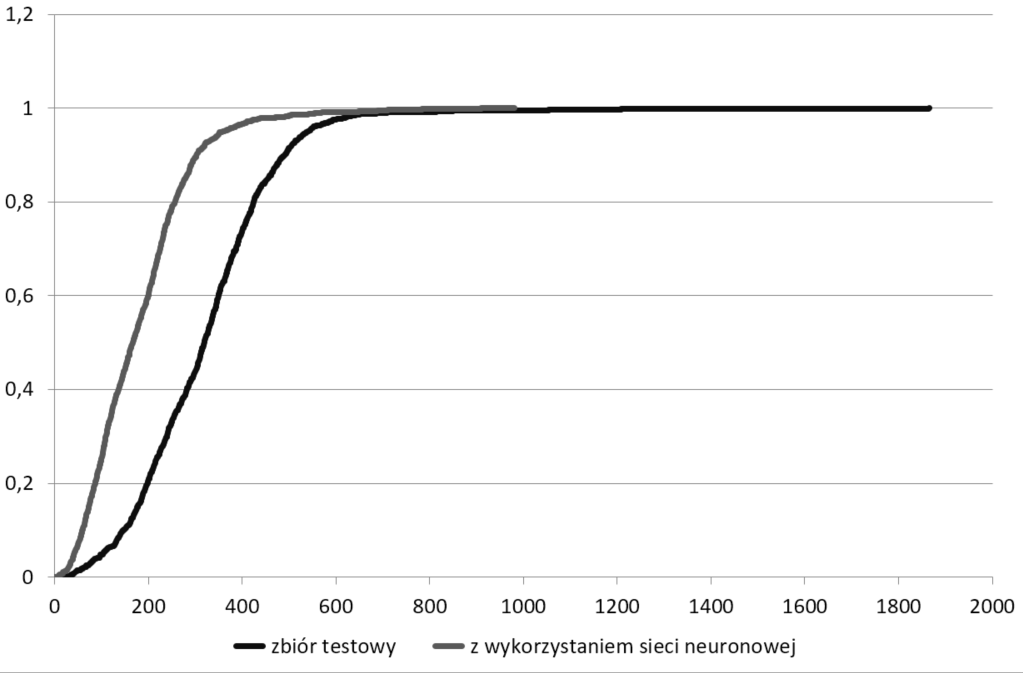
\includegraphics[width=1\textwidth]{{Wykresy/dystrybuanta.png}}
	\caption{Porównanie dystrybuant błędu pomiaru}
\end{figure}


\section{Kod źródłowy programu}

Program został napisany w języku $Java$ z wykorzystaniem narzędzia $Maven$ \cite{Maven}, służącego do automatyzacji budowy oprogramowania. Import danych oraz generowanie raportów w formacie $xlsx$ zaimplementowano z wykorzystaniem biblioteki $poi-ooxml$ \cite{Excel}.\newline

Kod źródłowy programu dostępny w repozytorium $GitHub$ \cite{Repo}.



\begin{thebibliography}{1}
\bibitem{zadanie} 
Treść zadania drugiego\newline
\textit{https://ftims.edu.p.lodz.pl/mod/page/view.php?id=73137}. 
\bibitem{Maven} 
Narzędzie Maven\newline
\textit{https://maven.apache.org/}. 
\bibitem{Excel} 
Biblioteka poi-ooxml\newline
\textit{https://mvnrepository.com/artifact/org.apache.poi/poi-ooxml}.
\bibitem{Repo} 
Kod źródłowy programu\newline
\textit{https://github.com/Walducha1908/sise2}. 
\end{thebibliography}

\end{document}
